\documentclass[ENG]{TFUOC}

\usepackage{graphicx}
\usepackage{float}
\usepackage{tikz}
\usepackage{booktabs}
\usepackage{array}
\usepackage{multirow}
\usepackage{amsmath}
\usetikzlibrary{arrows.meta,shapes.geometric,positioning,fit,backgrounds,calc}

%Introduce Work Data
\title{Analítica avanzada sobre datos de plataformas VOD y generadores de contenidos en redes sociales}
\titcrt{Analítica de plataformas VOD} %Short title to appear in header
\author{Pablo Jiménez Cruz}
\date{October 2026}


\nomPDC{Francesc Julbe López}
\nomPRA{Appoint Responsible Teaching Staff}
\titulac{Master in Data Science}
\area{Data Science}
\idioma{English}
\credits{12}
\parcla{artificial intelligence, video podcasts, YouTube analytics, automatic speech recognition, speaker diarization, video chaptering, highlight detection, local machine learning}

\licenc{ccBy}

%%%%%%%%%%
% Summary in language

\abstractenglish{
This Final Master's Project proposes the design and evaluation of a self-hosted platform that assists producers of YouTube video podcasts. The platform will automate post-production tasks (transcription, speaker identification, chapters, descriptions and short clips) and will support editorial decisions, such as choosing clips, titles and thumbnails, with models trained on real audience data obtained from the official YouTube APIs. All models will run locally on consumer hardware. The project will evaluate whether these trained models improve on simple baseline methods.
}

\begin{document}

\estructura

\tableofcontents

\renewcommand{\thesection}{\arabic{section}}

%==========================================================
\section{Title}
%==========================================================

\textbf{Analítica avanzada sobre datos de plataformas VOD y generadores de contenidos en redes sociales} (Advanced analytics on VOD platform data and social-media content creators).

The title refers to the main subject of the work: the analysis of data from a video-on-demand (VOD) platform, YouTube, to support content creators, specifically producers of video podcasts. The software developed in the project will be called \textit{YouTube Suite}.

%==========================================================
\section{Keywords}
%==========================================================

artificial intelligence, video podcasts, YouTube analytics, automatic speech recognition, speaker diarization, video chaptering, highlight detection, local machine learning.

%==========================================================
\section{Summary of the proposal}
%==========================================================

\textbf{Subject.} The project deals with video podcasts published on YouTube: long conversations, usually between one and three hours long, that must be packaged with subtitles, chapters, a description, a title, a thumbnail and several short vertical clips before they reach their audience. Preparing this material is slow and repetitive, and the most important decisions (which moments to clip, which title and thumbnail to use) are usually taken by intuition.

\textbf{What the project aims to achieve.} The goal is to build and evaluate \textit{YouTube Suite}, a platform where a producer uploads an episode and runs a set of AI tools on it: transcription and subtitles, speaker diarization, chapter generation, generation of descriptions and title suggestions, detection of the most relevant moments and automatic creation of short clips, and scoring of titles, thumbnails and clip openings. A data pipeline will collect public data from podcast channels and private audience data from the author's own channel, which will be used to train some of these models. The whole platform will run on the author's own computer, without paid cloud services.

At the end of the project, the expected result is a working and tested platform, together with a quantitative evaluation that shows whether the models trained on real data improve on simple baseline methods.

%==========================================================
\section{Justification}
%==========================================================

VOD platforms have become the main channel to distribute audiovisual content, and podcasts are increasingly recorded and published as video on YouTube. On these platforms, what each user sees is decided by recommendation systems that optimise signals such as watch time and click-through rate (CTR) \cite{recommender_systems_streaming, vod_bigdata}. For this reason, the reach of an episode depends not only on its content but also on its packaging: subtitles, chapters, title, thumbnail and short clips.

\textbf{Relevance for society.} Most podcasts are produced by small teams or by individuals, for whom preparing this material is a large share of the work. The tools available today are paid cloud services that solve isolated tasks and require uploading unpublished recordings to third parties. A free, local and integrated alternative would reduce the cost of entry for independent creators, protect the privacy of the people who take part in the episodes and improve accessibility through subtitles.

\textbf{Relevance for the scientific field.} The project touches several open problems in data science:
\begin{itemize}
\item \textit{Video chaptering}: the best current results are obtained with large language models \cite{ventura2025chapterllama}. It is not known how close a small model trained on public data \cite{yang2023vidchapters} can get on consumer hardware, nor how well it works in Spanish.
\item \textit{Highlight detection}: most methods are visual \cite{apostolidis2021survey}, while in a podcast the interesting content is in the speech. Obtaining labels is the main difficulty \cite{sul2023mrhisum}.
\item \textit{Engagement prediction}: YouTube does not publish CTR, so it can only be obtained from one's own channel \cite{yt_data_api}. Learning from a small and slowly growing set of real labels is a challenge in itself, which suggests ranking approaches \cite{burges2005ranknet}.
\end{itemize}

%==========================================================
\section{Motivation}
%==========================================================
% TODO (author): personalise this section with your own experience and reasons.

The first motivation is a personal interest in the production of video podcasts, and the observation that a large part of the time needed to publish an episode is spent on mechanical tasks that current AI models can solve, while the decisions that matter most are still taken without data.

The second motivation is academic: the project covers the whole life cycle of a data-science project studied in the master's degree, from the identification and capture of data (APIs and public datasets) to storage, modelling, evaluation and presentation of results in a real application.

Finally, there is a personal interest in showing that useful AI tools can be built and run locally, on modest hardware and without per-use costs.

%==========================================================
\section{Objectives}
%==========================================================

\textbf{What do I want to do?} Build a platform that automates the post-production of video podcasts and that learns from the performance of the published content.

\textbf{What do I want to verify or contribute?} Whether local models, trained on public and own-channel data, can do these tasks with useful quality on consumer hardware, and whether they improve on simple baseline methods.

\textbf{Scope.} The project includes the tools listed in the summary, the collection of public data from a selected list of podcast channels and of private data from a single channel (the author's own), and a web interface. It does not include automatic publication on YouTube (every result is reviewed by a person), a service for several users or channels, the use of image or audio as input for the relevance model, or translation. The objectives are orientative and will be refined in the next activities.

\subsection{Hypothesis (main objective)}

\textit{A self-hosted platform running on consumer hardware can automate the post-production of a YouTube video podcast, and models trained on public and own-channel data outperform the simple baseline methods they replace.}

\subsection{Partial objectives (research questions)}

\begin{enumerate}
\item[\textbf{O1}] Build the base of the platform (data storage, job processing and web interface) and integrate transcription and speaker diarization.
\item[\textbf{O2}] Develop a chapter generator for English and Spanish and compare it with an unsupervised baseline method \cite{hearst1997texttiling}.
\item[\textbf{O3}] Generate descriptions and title suggestions with a language model executed locally.
\item[\textbf{O4}] Develop a model that scores the relevance of each moment of an episode and use it to create short clips automatically.
\item[\textbf{O5}] Build a pipeline that collects public data from podcast channels and private audience data from the author's channel.
\item[\textbf{O6}] Develop models that score titles, thumbnails and clip openings, and retrain them as real data accumulates.
\end{enumerate}

These objectives lead to the following research questions:
\begin{enumerate}
\item[\textbf{RQ1}] Can all the required models run on a computer with a 3\,GB GPU in a reasonable time per episode?
\item[\textbf{RQ2}] Does a small chapter model trained on public data outperform an unsupervised baseline, and does it work in Spanish?
\item[\textbf{RQ3}] Does a relevance model trained with audience data choose better clips than a heuristic method?
\item[\textbf{RQ4}] Is the data available from a single channel and from public sources, within the API limits, enough to train useful models for titles, thumbnails and clip openings?
\end{enumerate}

%==========================================================
\section{Methodology}
%==========================================================

\subsection{Research strategy}

According to the classification of Oates \cite{oates2006researching}, the main strategy will be \textbf{design and creation}: the contribution of the project is a new IT artefact (the platform and its models), whose construction and evaluation produce knowledge about the problem \cite{hevner2004design}. To answer the research questions about the models, an \textbf{experiment} strategy will be used: each model will be compared with a baseline method on data not used for training.

\textbf{Data generation techniques.} The data will be mainly \textit{quantitative}:
\begin{itemize}
\item A public dataset of YouTube videos with chapters and transcripts \cite{yang2023vidchapters}.
\item Public data (metadata and statistics) from a selected list of podcast channels, and private audience data (retention, impressions and CTR) from the author's channel, obtained through the official YouTube APIs \cite{yt_data_api}.
\item Measurements: evaluation metrics of each model, and processing time and memory use.
\end{itemize}
A small \textit{qualitative} part will consist of the author's review of the generated titles and clips on real episodes.

\textbf{Tools.} Python and PyTorch for data analysis and modelling, Jupyter notebooks for the experiments, PostgreSQL as database, and Git for version control. No statistical packages such as SPSS or MINITAB are needed.

\subsection{Work methodology and key concepts}

\textbf{Possible strategies.} Three strategies were considered: (1)~combining existing commercial services, which is fast but has per-use costs, requires uploading recordings to third parties and does not allow training with one's own data; (2)~adapting an existing open-source tool, which only covers isolated tasks; and (3)~developing a new integrated product that reuses mature open models where they exist and trains new models where they do not.

\textbf{Chosen strategy.} The third one, \textbf{developing a new product}, because it is the only one that allows all the tools to share the same data, keeps all processing local and allows the models to be trained with the creator's own data, which is the core of the hypothesis.

\textbf{Development process.} An incremental methodology will be followed, based on small milestones. Each milestone will have three phases: planning (a short design and test plan), development and testing (new tests and a check that earlier parts still work). Important technical decisions will be documented as they are taken, and model development will be done as documented and reproducible experiments. The order of the milestones guarantees that a working version of the product exists from the beginning and grows step by step.

\textbf{Resources.} The author's desktop computer (with a 3\,GB GPU), open-source software and models, the free quotas of the YouTube APIs, and the author's own channel and episodes as test material.

%==========================================================
\section{Ethical and global commitment competence (CCEG) and Sustainable Development Goals (SDG)}
%==========================================================

The three dimensions of the CCEG will be considered at the design stage (described here), during development and in the conclusions of the project.

\subsection*{Sustainability}

The main environmental impact of the project is the energy consumed when running and training models. It will be reduced by using small models that fit an existing computer instead of new hardware or large cloud clusters, by computing each intermediate result (for example, the transcript) only once and reusing it in all the tools, and by collecting data with a small number of grouped API requests. During development, the resource usage of each model will be measured, and its impact will be discussed in the conclusions. This is related to SDG~9 (Industry, innovation and infrastructure) and SDG~12 (Responsible consumption and production).

\subsection*{Ethical behaviour and social responsibility}

The main ethical risks are optimising content only for engagement and creating clips that take statements out of context. To reduce them, the platform will never publish anything automatically: every result will be reviewed by a person, and the scoring models will show the reasons behind their scores. Reducing repetitive work for small creators while keeping editorial control in human hands is related to SDG~8 (Decent work and economic growth).

\textbf{Ethics and personal data protection protocol.} The project will process personal data (the voices and words of the people who take part in the episodes and the audience data of a channel), so it will follow the GDPR \cite{gdpr2016} and the Spanish Organic Law 3/2018 \cite{lopdgdd2018}:
\begin{itemize}
\item \textit{Consent and transparency}: the people who take part in the episodes will be informed and will give their consent before their recordings are used. Private channel data will only be accessed with the explicit authorisation of the channel owner.
\item \textit{Minimisation}: only the data needed will be collected, and only through the official APIs and according to their terms of use. No data about individual viewers will be collected.
\item \textit{No identification}: speakers will be labelled anonymously (speaker 1, speaker 2, \dots); no identity, gender or age will be inferred from voices.
\item \textit{Security}: all data will be stored and processed locally and will not be sent to external services. Access credentials will be stored encrypted.
\item \textit{Deletion}: any episode and all the data derived from it can be deleted on request.
\item \textit{Public datasets}: they will only be used to train models and will not be redistributed.
\end{itemize}
The report will only show aggregated results. The project is not carried out in a company, so no collaboration or confidentiality agreement is needed.

\subsection*{Diversity, gender and human rights}

Speech and language models may work worse for some accents, languages or voices because of biases in their training data. To detect this, the chapter models will be evaluated separately in English and in Spanish, and speaker labels will be anonymous. Automatic subtitles improve accessibility for deaf and hard-of-hearing people, and supporting Spanish, a language with little public data for this task, is related to SDG~10 (Reduced inequalities).

%==========================================================
\section{Project planning}
%==========================================================

The design of the project and the base of the platform (objective O1) were completed before this proposal. Table~\ref{tab:planning} lists the tasks from now on, with their duration, start and end dates and dependencies, and Figure~\ref{fig:gantt} shows them as a Gantt chart. The data-collection track (T5--T7) depends only on the base of the platform, so it can run in parallel with the tools.
% TODO (author): check the delivery dates of the course activities (PECs) and the defence against the official UOC calendar.

\begin{table}[H]
\centering
\caption{Tasks, duration, dates and dependencies.}
\label{tab:planning}
\small
\begin{tabular}{@{}lp{7.6cm}lll@{}}
\toprule
\textbf{ID} & \textbf{Task} & \textbf{Duration} & \textbf{Dates} & \textbf{Depends on} \\
\midrule
T1 & Chapter generator (O2) & 1 week & Oct 13--19 & -- \\
T2 & Descriptions and title suggestions (O3) & 1 week & Oct 20--26 & T1 \\
T3 & Relevance model, first version (O4) & 1 week & Oct 27--Nov 2 & -- \\
T4 & Automatic short clips (O4) & 2 weeks & Nov 3--16 & T3 \\
T5 & Public data collection (O5) & 2 weeks & Oct 20--Nov 2 & -- \\
T6 & Private audience data of the own channel (O5) & 2 weeks & Nov 3--16 & T5 \\
T7 & Real CTR and impressions data (O5) & 2 weeks & Nov 17--30 & T6 \\
T8 & Global testing of the tools & 1 week & Nov 17--23 & T1--T4 \\
T9 & Title, thumbnail and clip-opening scoring (O6) & 2 weeks & Nov 24--Dec 7 & T4, T7 \\
T10 & Model retraining with real data (O4, O6) & 2 weeks & Dec 8--21 & T3, T7, T9 \\
T11 & Final experiments and evaluation & 1.5 weeks & Dec 22--31 & T8, T10 \\
\midrule
D1 & Proposal (this document) & 1 week & Oct 13--19 & -- \\
D2 & State of the art & 2 weeks & Oct 20--Nov 2 & D1 \\
D3 & Writing of the report (incremental) & 8.5 weeks & Nov 3--Dec 31 & D2 \\
D4 & Final report & 1.5 weeks & Jan 1--10 & D3, T11 \\
D5 & Presentation and defence & 2 weeks & Jan 11--24 & D4 \\
\bottomrule
\end{tabular}
\end{table}

\begin{figure}[H]
\centering
\resizebox{\textwidth}{!}{%
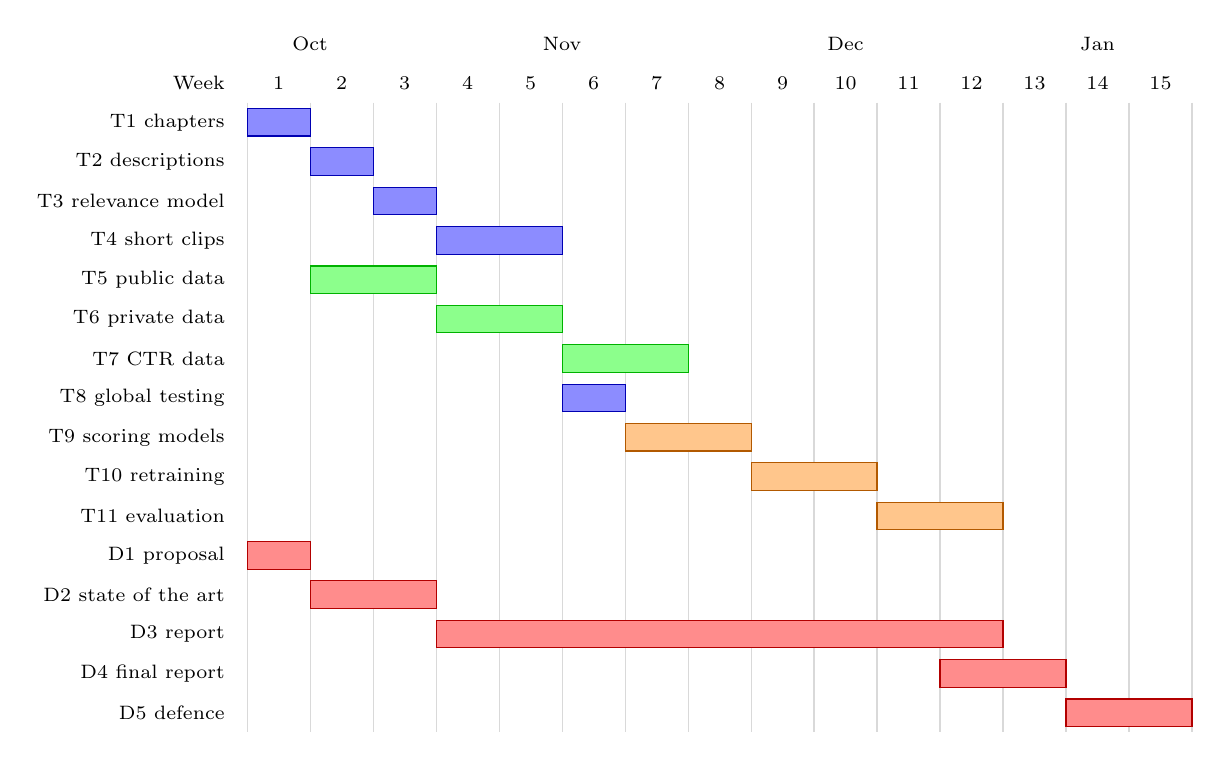
\begin{tikzpicture}[x=0.8cm, y=0.5cm]
  % week grid (week 1 starts on 13 October 2026)
  \foreach \w in {0,...,15} { \draw[gray!30] (\w,0.5) -- (\w,-15.5); }
  \foreach \w in {1,...,15} { \node[font=\scriptsize] at (\w-0.5,1) {\w}; }
  \node[font=\scriptsize, anchor=east] at (-0.2,1) {Week};
  \node[font=\scriptsize] at (1,2) {Oct};
  \node[font=\scriptsize] at (5,2) {Nov};
  \node[font=\scriptsize] at (9.5,2) {Dec};
  \node[font=\scriptsize] at (13.5,2) {Jan};
  % rows: y / label / start week / end week / colour
  \foreach \y/\lab/\s/\e/\c in {
      0/T1 chapters/1/1/blue,
      1/T2 descriptions/2/2/blue,
      2/T3 relevance model/3/3/blue,
      3/T4 short clips/4/5/blue,
      4/T5 public data/2/3/green,
      5/T6 private data/4/5/green,
      6/T7 CTR data/6/7/green,
      7/T8 global testing/6/6/blue,
      8/T9 scoring models/7/8/orange,
      9/T10 retraining/9/10/orange,
      10/T11 evaluation/11/12/orange,
      11/D1 proposal/1/1/red,
      12/D2 state of the art/2/3/red,
      13/D3 report/4/12/red,
      14/D4 final report/12/13/red,
      15/D5 defence/14/15/red} {
    \node[font=\scriptsize, anchor=east] at (-0.2,-\y) {\lab};
    \fill[\c!45, draw=\c!70!black] (\s-1,-\y-0.35) rectangle (\e,-\y+0.35);
  }
\end{tikzpicture}}
\caption{Gantt chart from 13 October 2026. Blue: tools; green: data collection; orange: trained models and evaluation; red: course deliverables.}
\label{fig:gantt}
\end{figure}

\textbf{Risks.} Three tasks have a higher risk and have extra time: the automatic clips (T4), whose quality is subjective and hard to test; the real CTR data (T7), which comes from the newest and least documented API and arrives with a delay; and the retraining (T10), because there is no guarantee that the trained models will beat the baseline methods. In that case, the baseline methods will remain in use and the result will be reported. If there are delays, the priority will be the tools first, then data collection, and finally the trained models.

%==========================================================
% Bibliography (numeric, by order of appearance)
%==========================================================
\bibliographystyle{IEEEtran}
\bibliography{references}

\end{document}
